\chapter{ Le  Machine Learning}
\label{Le Machine Learning}
\thispagestyle{fancy}

\section{Généralités sur le Machine Learning}
\label{Le Machine Learning: Généralités sur le Machine Learning}
Le Machine Learning (traduire par apprentissage automatique) est une ramification de l'intelligence artificielle. Cependant, son statut de subdivision n'informe en rien sur l'étendu des notions contenues dans cette matière scientifique. Son champ d'étude est vaste et en perpétuelle évolution. Les solutions offertes par cette discipline permettent d'étudier toute sortes de données et d'automatiser une multitude de systèmes. L'apprentissage automatique rencontre un succès croissant qui est corrélé avec l'essor des nouvelles technologies et l'automatisation de l'analyse de volumes conséquents de données utilisateurs (Big Data). Les applications sont donc multiples. En voici quelques exemples:  

\begin{itemize}
	\item Algorithmes des moteurs de recherches (Google Deep Dream, Google TensorFlow)
	\item Analyse boursière
	\item Analyse de rapports d'erreurs
	\item Reconnaissance vocale, biométrie, reconnaissance d'écriture
	\item Robotique (vision, mouvements, prise de décision, etc.)
	\item Neurosciences 
\end{itemize}

\subsection{Définition et principe général du Machine Learning}
\label{Le Machine Learning: Généralités sur le Machine Learning: Définition et principe général}
Le champ d'étude et d'application du Machine Learning étant immense, on propose de redéfinir cette notion en l'adaptant à la résolution de notre problématique (i.e. automatiser l'analyse d'incidents révélés lors du filtering test).
On offre ici deux définitions de l'apprentissage automatique: une première dite "High Level" qui le caractérise de manière générale et une seconde qui reflète sa dimension algorithmique. 

\begin{description}
	\item[High Level]: Le Machine Learning permet à un système d'évoluer grâce à un processus d'apprentissage et ainsi de remplir des tâches qu'il est difficile, voir impossible, de remplir par d'autres moyens algorithmiques plus classiques. 
	\item[Mathématique] Le Machine Learning fourni les outils pour prédire une/des donnée(s) de sortie Y à partir des données d'entrée X via un processus d'apprentissage. 
\end{description}
 
 De nombreuses autres définitions existent, mais elles ne correspondent pas à la dimension recherchée dans le cadre de ce projet.
 
Au regard des deux définitions stipulées ci-dessus, on peut définir le principe de base de l'apprentissage automatique sous la forme d'un schéma bloc 	ref{fig:Schéma fonctionnel haut niveau du Machine Learning}.

\begin{figure}[h]
	\centering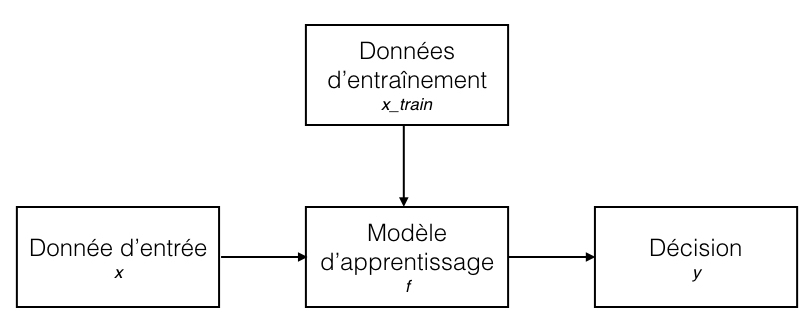
\includegraphics[height=5cm]{images/ML_high_level.jpeg}
	\caption{Schéma fonctionnel haut niveau du Machine Learning}
	\label{fig:Schéma fonctionnel haut niveau du Machine Learning}
\end{figure}

L'apprentissage automatique peut donc être vu dans sa globalité comme un processus composé de deux étapes successives : 
\begin{enumerate}
		\item [Apprentissage]
		 \begin{enumerate}
			\item  Un ensemble de données est présenté au système (X\_train).
			\item A partir de ces informations, le système (f) apprend - s'entraîne- afin d'être par la suite en capacité de prendre décision vis à vis de la tâche qui lui sera demandée. 
		\end{enumerate}
		
		\item [Prise de décision] 
		\begin{enumerate}
			\item  On a en entrée du système une ou des donnée(s) brutes (X).  
			\item Cette donnée est traitée et analysée par le système.
			\item En sortie, une décision est prise quant à la tâche demandée (Y). 
		\end{enumerate}
\end{enumerate}

\subsubsection{Un exemple concret}
\label{Le Machine Learning: Généralités sur le Machine Learning: Définition et principe général:un exemple concret}
Afin de présenter de manière plus concrète le processus fonctionnel haut niveau d'un algorithme d'apprentissage, on présente l'exemple suivant:

\textit{On cherche à déterminer à quelle période de l'année nous nous trouvons (i.e. printemps, été, automne ou hiver) à partir de l'humidité, la température et la pression atmosphérique d'aujourd'hui. \\
	La première étape de notre processus sera donc d'entrainer notre système afin que celui-ci soit en mesure de prendre une décision vis à vis des données qu'on lui présentera en entrée (i.e. l'humidité, la température et la pression atmosphérique d'aujourd'hui). \\
	Une fois le système entrainé, on attend que celui-ci ai ce type de comportement : \\
	On présente en entrée de mon système une température de -2 degrés, une pression atmosphérique de 1030hPa et un taux d'humidité de 81\%. La réponse attendue en sortie du système est: hiver}

On peut adapter le schéma fonctionnel haut niveau du Machine Learning à notre exemple \ref{fig:Schéma fonctionnel haut niveau du Machine Learning, l'exemple prévision saisonnière}. 

\begin{figure}[h]
	\centering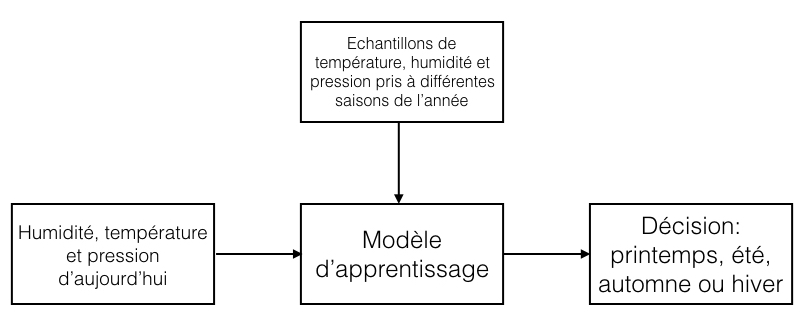
\includegraphics[height=5cm]{images/ML_high_level_expl.jpeg}
	\caption{Schéma fonctionnel haut niveau du Machine Learning, l'exemple de la prévision saisonnière}
	\label{fig:Schéma fonctionnel haut niveau du Machine Learning, l'exemple prévision saisonnière}
\end{figure}

Pour caractériser et  désigner plus précisément les différents éléments de notre système, on présente ci-dessous le champs lexical utilisé dans le domaine du Machine Learning:

\subsubsection{Lexique} 
\begin{description}
	\item [les features] Le type de données présenté en entrée. \\
	\textit{La température, la pression atmosphérique et l'humidité.}
	\item [échantillons ou exemples] Les données permettant d'entrainer le système (x\_train). \\
	\textit{De nombreux échantillons de température, pression atmosphériques et humidité pris à différents périodes de l'année, sur plusieurs années.}
	\item [le modèle d'apprentissage] Le cœur du système décisionnel (f).
	\item [La décision] La sortie ou réponse du système (Y) \\
	\textit{Printemps, été, automne ou hiver.}
\end{description}

\subsection{Les exemples}
\label{Le Machine Learning: Généralités sur le Machine Learning: Les données}
Les exemples correspondent aux données utilisées pour entraîner mon algorithme d'apprentissage. On parle également d'échantillons. Celles-ci sont regroupées en "features" (terme anglais, traduire par caractéristiques). 
Pour reprendre l'exemple cité précédemment \ref{Le Machine Learning: Généralités sur le Machine Learning: Définition et principe général:un exemple concret}, nos données sont regroupées en 3 features: la température, l'humidité et la pression atmosphérique. On données sont donc structurées de la manière suivante: 

\begin{equation}
\begin{blockarray}{cccc}
& température (\degres C) & humidite (\%) & pression(HPa) \\
\begin{block}{c(ccc)}
Exemple_1 & -10 & 85 & 1023 \\
Exemple_2 & 15 & 80 & 1020 \\
Exemple_3 & 23 & 65 & 1015 \\
... & ... & ... & ... \\
Exemple_n & 10 & 81 &  1032 \\
\end{block}
\end{blockarray}
\end{equation}

\subsubsection{Différents types de données}
Il existe deux types de données: les données labellisées et non labellisées.
\begin{itemize}
	\item Les données labellisées correspondent à des exemples corrélés à une sortie - un label - connue.
	\item Les données non labellisées ne sont quant à elles pas associées à une sortie. 
\end{itemize}

Pour reprendre l'exemple précédent \ref{Le Machine Learning: Généralités sur le Machine Learning: Définition et principe général:un exemple concret}, on a les jeux de données suivants: 

\textbf{Données labellisées} 
\begin{equation}
\begin{blockarray}{ccccc}
& température (\degres C) & humidite (\%) & pression(HPa) \\
\begin{block}{c(ccc)c}
Exemple_1 & -10 & 85 & 1023 & hiver\\
Exemple_2 & 15 & 80 & 1020 & automne\\
Exemple_3 & 23 & 65 & 1015 & ete \\
... & ... & ... & ... \\
Exemple_n & 10 & 81 &  1032 & printemps\\
\end{block}
\end{blockarray}
\end{equation}
On connait la sortie qui correspond aux données d'entrée, i.e. que on sait à quelle période de l'année les échantillons ont été prélevé.
 
\textbf{Données non labellisées} 
\begin{equation}
\begin{blockarray}{ccccc}
& température (\degres C) & humidite (\%) & pression(HPa) \\
\begin{block}{c(ccc)c}
Exemple_1 & -10 & 85 & 1023 & ??\\
Exemple_2 & 15 & 80 & 1020 & ??\\
Exemple_3 & 23 & 65 & 1015 & ?? \\
... & ... & ... & ... \\
Exemple_n & 10 & 81 &  1032 & ??\\
\end{block}
\end{blockarray}
\end{equation}
On ne connait pas la sortie qui correspond aux données d'entrée, i.e. que on \emph{ne} sait \emph{pas} à quelle période de l'année les échantillons ont été prélevé. 

\subsection{La décision}
\label{Le Machine Learning: Généralités sur le Machine Learning: La décision}
La sortie de notre système peut être également nommé décision. Toujours selon notre exemple \ref{Le Machine Learning: Généralités sur le Machine Learning: Définition et principe général:un exemple concret}, cela correspond au choix fait par l'algorithme entre les différentes saisons: printemps, été, automne et hiver.  

\subsubsection{Différents types de sorties}
Il existe différents types de sortie: les sorties continues et discrètes.

\begin{description}
	\item [Les sorties continues] peuvent prendre n'importe quelle valeur. \\
	 $y \in R$ \\
	 Déterminer l'évolution de la température en fonction des échantillons enregistrés les mois précédents correspond à une sortie continue.
	\item [Les sorties discrètes] ne peuvent prendre que des valeurs prédéterminées. \\
	 $y \in {1, 2, 3, ...,C}$ \\
	 L'exemple \ref{Le Machine Learning: Généralités sur le Machine Learning: Définition et principe général:un exemple concret} a une sortie discrète. En effet, la sortie ne peut prendre que des valeurs prédéterminées: printemps, été, automne et hiver.
\end{description}


\subsection{Le modèle}
\label{Le Machine Learning: Généralités sur le Machine Learning: Le modèle}
Il existe différents types d'apprentissages. Le choix d'un modèle en particulier est influencé par le type d'exemples que l'on a en entrée du système et du type de décision que l'on souhaite obtenir en sortie. Nous nous intéresserons à différentes catégories d'apprentissages automatiques: 
\begin{itemize}
	\item Les apprentissages supervisés et non-supervisés. Cette caractéristique dépend du type d'exemples que l'on a en entrée du système.
	\item Les régression ou les classifications. Cette caractéristique dépend du type de sortie que l'on souhaite obtenir . 
\end{itemize}

\subsubsection{apprentissage supervisé et non supervisé} 
\label{Le Machine Learning: Généralités sur le Machine Learning: Le modèle: apprentissage supervisé et non supervisé}
L'apprentissage supervisé nécessite d'avoir des données labellisées en entrée, i.e. que l'on connait le type de décision que l'on aura en sortie du système en fonction des exemples en entrée: il y'a une corrélation entre la sortie et l'entrée. C'est cette notion qui s'exprime au travers du terme \emph{supervisé}. 
L'apprentissage non supervisé s'appuie quant à lui sur l'utilisation d'une base de donnée non labellisée pour son apprentissage, i.e qu'on ne connait pas le type de décision associé aux exemples en entrée. Dans le cas d'un apprentissage non supervisé, pour parvenir à prendre une décision, l'algorithme devra diviser ce groupes de données hétérogènes en sous-groupes homogènes d'informations similaires. On appelle ces subdivisions des \emph{clusters}.
Afin de matérialiser les différences entres les deux méthodes et les applications possibles pour chacune d'elles, on propose deux exemples \ref {tab: Comparaison des différentes méthodes d'apprentissage}.

\begin{table}[h]
	\begin{tabular}{ | p {2.5cm} | p {6cm} | p {6cm} |}
	\hline
	 & apprentissage supervisé & apprentissage non supervisé \\
	\hline
	\begin{tabular}{c} exemple n\degres1:\\apprendre aux \\ humains \end{tabular}  &
	 Une institutrice souhaite apprendre à ses élèves à différencier un chat d'un chien: c'est la décision qu'on attend d'eux. Pour ce faire, l'éducatrice leur montre différentes photographies de chiens et de chats: ce sont les exemples utilisés pour l'apprentissage. Ces exemples peuvent être segmentés en différentes caractéristiques, comme la taille de l'animal, sa couleur, la longueur du poil, etc: il s'agit des features. Lorsque que l'institutrice leur présente les différentes images, elle stipule clairement si il s'agit d'un chien ou d'un chat: il y'a donc une corrélation entre l'entrée et la sortie de l'apprentissage, il s'agit d'un apprentissage supervisé (figure \ref{fig:Comparaison d'un apprentissage supervisé et non supervisé dans le cadre de l'exemple "apprendre aux humains"},a).&
	 On retrouve cette même institutrice donnant à ses élèves le même exercice à la différence que, contrairement à précédemment, lorsque qu'elle présente les différentes images, elle \emph{ne} stipule \emph{pas} la race de l'animal: il n'y a donc aucune corrélation entre l'entrée et la sortie de l'apprentissage, il s'agit donc d'un apprentissage non supervisé. Pour réussir cet exercice, les enfants devront donc regrouper les animaux en s'appuyant sur leurs similitudes physiques, i.e. leurs features (e.g. taille de l'animal, sa couleur, longueur du poil, etc.). Les élèves ne connaitrons certes pas le nom des deux animaux, mais ils auront su les différencier. C'est la même approche qui est réalisé en apprentissage automatique non supervisé (figure \ref{fig:Comparaison d'un apprentissage supervisé et non supervisé dans le cadre de l'exemple "apprendre aux humains"}, b). \\
	\hline 
	\begin{tabular}{c} exemple n\degres2:\\la météo \ref*{Le Machine Learning: Généralités sur le Machine Learning: Définition et principe général:un exemple concret}\end{tabular} &
	 On reprend l'exemple dans lequel on souhaite prendre une décision quant à la période de l'année à laquelle on se trouve actuellement, en fonction des features humidité, température et pression atmosphérique. Pour se faire, on prélève des échantillons à différentes périodes de l'année en notant à quelle saison ces données ont été prélevées: se sont des exemples labellisées, i.e. il y'a une corrélation entre les données et la sortie du système. Il s'agit donc d'un apprentissage supervisé (figure \ref{fig:Comparaison d'un apprentissage supervisé et non supervisé dans le cadre de l'exemple prévision saisonnières}, a). &
	On reprend le même problème mais cette fois-ci on ne note pas la saison à laquelle les échantillons ont été prélevé. Pour résoudre le problème, l'algorithme doit donc associer les données les plus similaires entre elles et ainsi créer des groupes homogènes d'informations qui correspondront aux 4 décisions possibles (figure \ref{fig:Comparaison d'un apprentissage supervisé et non supervisé dans le cadre de l'exemple prévision saisonnières}, b). \\
	\hline
	\end{tabular}
	\caption[Comparaison des différents modèles d'apprentissage]{Comparaison de l'apprentissage supervisé et non supervisé par des exemples}
	\label {tab: Comparaison des différentes méthodes d'apprentissage}
\end{table}

%inverser les labels taille et longueur du pelage
\begin{figure}[h]
	\centering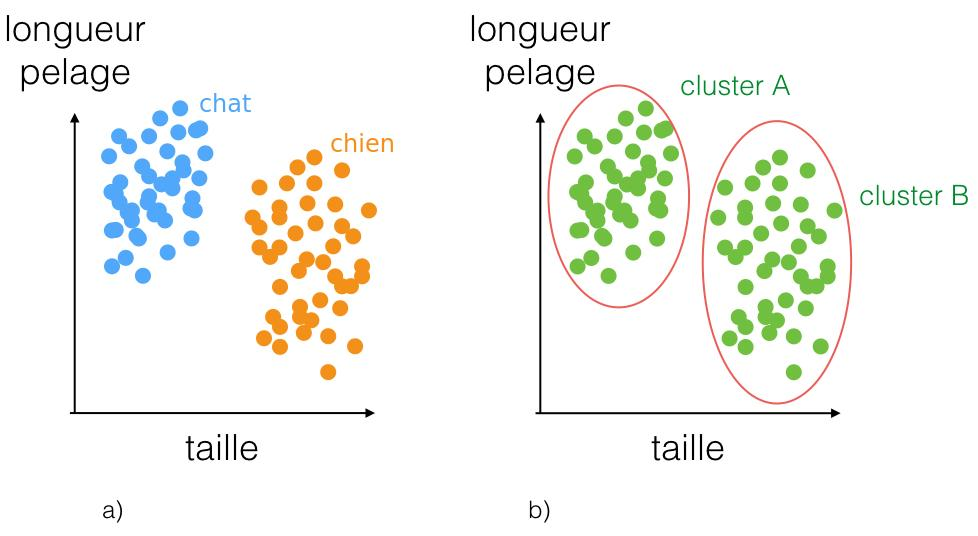
\includegraphics[height=7cm]{images/apprentissage_chat.jpeg}
	\caption[Comparaison d'un apprentissage supervisé et non supervisé dans le cadre de l'exemple "apprendre aux humains"]{Comparaison d'un apprentissage supervisé et non supervisé dans le cadre de l'exemple "apprendre aux humains". On observe sur la figure a) les différents exemples d'entrainement exprimés dans un repère composé des deux features "taille" et "longueur de pelage". On remarque qu'il y'a la formation de deux groupes de données homogènes: les animaux de taille globalement élevée avec un pelage court et les animaux de taille moindre avec un poil globalement plus long. Les données étant labellisées, on sait que le premier groupe correspond à des chiens et le deuxième à des chats.}
	\label{fig:Comparaison d'un apprentissage supervisé et non supervisé dans le cadre de l'exemple "apprendre aux humains"}
\end{figure}

\begin{figure}[h]
	\centering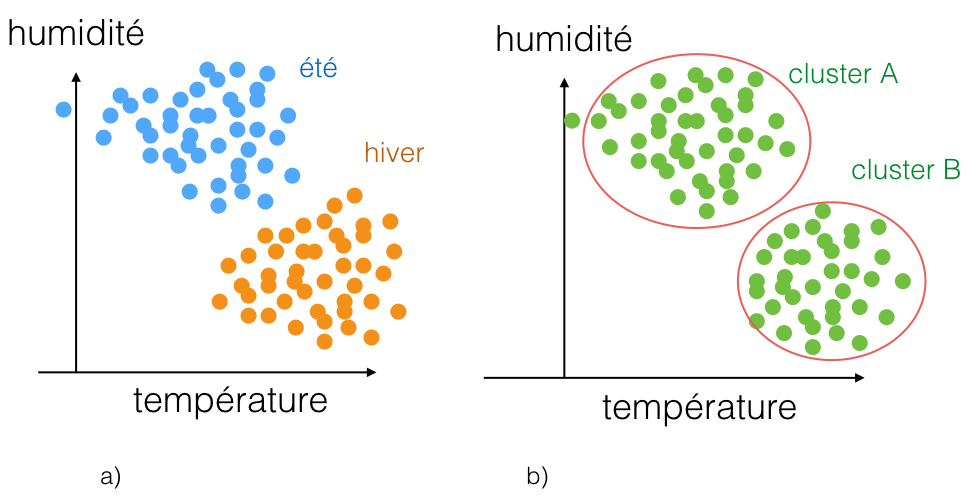
\includegraphics[height=7cm]{images/apprentissage_meteo.jpeg}
	\caption[Comparaison d'un apprentissage supervisé et non supervisé dans le cadre de l'exemple "prévisions saisonnières"]{Comparaison d'un apprentissage supervisé et non supervisé dans le cadre de l'exemple "prévisions saisonnières". On observe sur la figure a) les différents exemples d'entrainement exprimés dans un repère composé des deux dimensions (features) "humidité" et "température". On remarque qu'il y'a la formation de deux groupes de données homogènes: un où les échantillons sont pris lors de saisons globalement chaudes et sèches etc un autre où les échantillons sont enregistrés lors de périodes globalement froides et humides. Les données étant labellisées, on sait que le premier groupe correspond à l'été et l'autre groupe l'hiver.}
	\label{fig:Comparaison d'un apprentissage supervisé et non supervisé dans le cadre de l'exemple prévision saisonnières}
\end{figure}

Il existe deux types d'apprentissage supervisé: la régression et la classification.
%
%\subsubsection{Apprentissage supervisé: régression et classification} 
%\label{Le Machine Learning: Généralités sur le Machine Learning: Le modèle:Regression et classification}
% La régression est un type d'apprentissage avec lequel on souhaite obtenir une sortie continue. Dit de manière différente, la régression implique que l'on souhaite \emph{estimer} ou \emph{prédire} une réponse. 
%La classification est quant à lui un type d'apprentissage avec lequel on souhaite obtenir une sortie discrète, elle peut être vu comme un cas particulier de la régression où les valeurs à prédire sont discrètes. Formulé autrement, la classification implique que l'on souhaite classer un exemple parmi différentes. Afin de représenter concrètement les différences entre les deux méthodes et les applications possibles pour chacune d'elle, on propose un exemple.
%
%\begin{table}[h]
%	\begin{tabular}{ | p {7cm} | p {7cm} |}
%		\hline
%		régression & classification \\
%		\hline
%		On souhaite connaitre le temps (température et humidité) qu'il fera pendant les jours suivants. Pour cela, on s'appuie sur les différents échantillons de température et d'humidité enregistrés lors des mois et des années précédentes (exemples labellisés). Le fait de déterminer la température des jours suivants relève de la prédiction (figure \ref {tab: Comparaison des différentes catégories d'apprentissage supervisé}, a).  
%		 &  L'exemple de la prédiction saisonnière \ref{Le Machine Learning: Généralités sur le Machine Learning: Définition et principe général:un exemple concret} est bien un problème de classification: on cherche à classer notre donnée d'entrée parmi plusieurs groupes de données homogènes: printemps, été automne ou hiver (figure \ref {tab: Comparaison des différentes catégories d'apprentissage supervisé}, b). \\
%		\hline 
%	\end{tabular}
%	\caption[Comparaison des différentes catégories d'apprentissage supervisé]{Comparaison entre l'apprentissage supervisé de type régression et supervisé de type classification}
%	\label {tab: Comparaison des différentes catégories d'apprentissage supervisé}
%\end{table}
%
%\begin{figure}[h]
%	\centering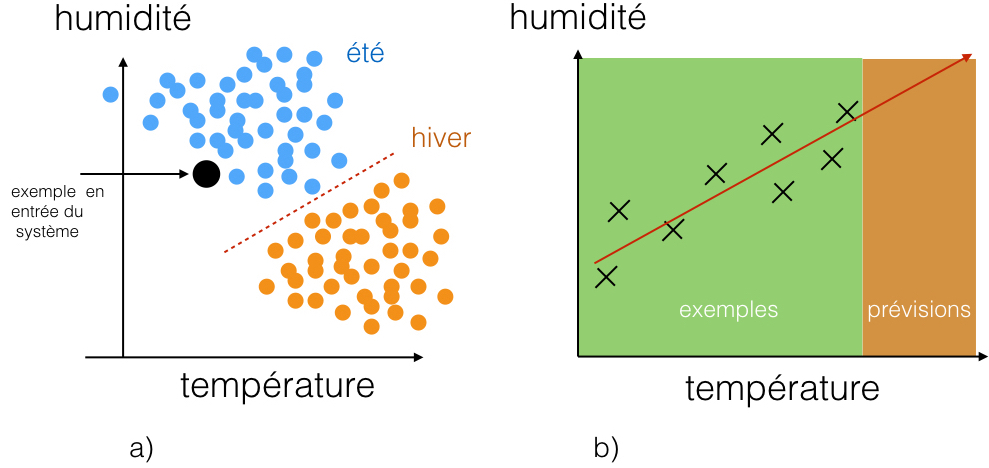
\includegraphics[height=7cm]{images/regression_class.jpeg}
%	\caption[Comparaison par l'exemple de la régression et la classification]{Comparaison par l'exemple de la régression et la classification. Sur la figure a), on observe deux jeux de données homogènes (été et hiver) s'exprimant dans un repères en deux dimensions (features humidité et température). Le but est ici de classer la donnée en entrée du système parmi ces deux ensembles, il s'agit donc d'un problème de classification. Dans la figure b), on observe une succession d'exemples exprimés dans un repère en deux dimensions (features température et humidité). On remarque une évolution globalement linéaire de ces exemples, nous permettant ainsi de prédire la température et l'humidité sur les prochains mois: il s'agit d'un problème de régression.}
%	\label{fig:Comparaison par l'exemple de la régression et la classification}
%\end{figure}
%
%\section{Les différents algorithmes d'apprentissage supervisé}
%\label{Le Machine Learning:Les différents algorithmes d'apprentissage supervisé}
%Il existe différents algorithmes d'apprentissage supervisés utilisés pour résoudre des problèmes de régression et de classification. 
%
%\subsection{La régression linéaire}
%\label{Le Machine Learning:Les différents algorithmes d'apprentissage supervisé: La regression linéaire}
%La régression linéaire cherche à expliquer une variable de sortie $Y$ par une fonction affine de $X$.  Cette fonction affine est appelée \emph{hypothèse} $h$. Exprimé autrement, on a un jeu de données $X$ auquel correspond un jeu de données $Y^$, on cherche les valeurs $\theta_1$ et $\theta_2$ permettant de "mapper" les données, tel que:
%
%\begin{equation}
%	h_\theta (x) = \theta_0 + \theta_1 x
%\end{equation}
%
%\subsubsection{Exemple de régression linéaire uni-variable}
%\label{Le Machine Learning:Les différents algorithmes d'apprentissage supervisé: La regression linéaire: Exemple de régression linéaire uni-variable}
%On souhaite déterminer le prix d'un logement en fonction de sa surface au sol en se basant sur les exemples de prix connus du parc immobilier. 
%La surface au sol est donc l'entrée $X$ de notre système et le prix la sortie $Y$. Soit le tableau \ref {tab:parc immobilier} les exemples $X$, on obtient la représentation graphique en figure 	\ref{fig:évolution du prix de l'immobilier en fonction de la surface}. Grâce à l'expression de l'hypothèse, on est capable de déterminer le prix d'un loyer en fonction de la surface au sol.  
%
%\begin{table}[h]
%	\begin{tabular}{ | p {7cm} | p {7cm} |}
%		\hline
%		taille (m^2) & prix (€) \\
%		\hline
%		2104&460
%		1416&232
%		1534&314
%		852&178
%		500&100
%		1012&212
%		126&75
%		1775&432
%		600&150
%		2114&510
%		1316&270
%		1634&334
%		\hline 
%	\end{tabular}
%	\caption[parc immobilier]{exemples du prix des logements en fonction de leur taille}
%	\label {tab:parc immobilier}
%\end{table}
%
%\begin{figure}[h]
%	\centering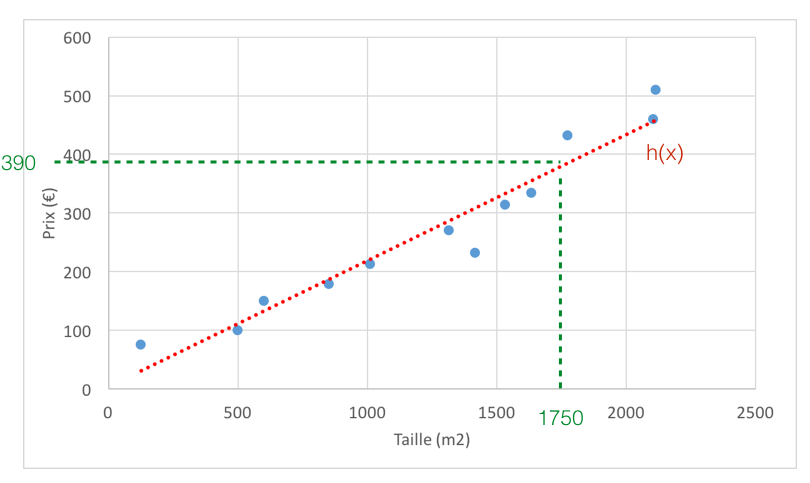
\includegraphics[height=7cm]{images/graph_immobilier.png}
%	\caption[évolution du prix de l'immobilier en fonction de la surface]{évolution du prix de l'immobilier en fonction de la surface. L'ensemble des données semble globalement évoluer de manière linéaire. Cette linéarité est représentée par l'hypothèse ($h(x)$). Grâce à celle-ci, on peut déterminer le prix d'un logement en fonction de sa superficie, et inversement. Par exemple, un appartement d'une surface de 1750 m^2 coutera aux alentours de 390 €.}
%	\label{fig:évolution du prix de l'immobilier en fonction de la surface}
%\end{figure}
%
%Cet exemple est dit uni-variable car un seul jeu de données $X$ (superficie) correspond à un jeu de données $Y^$ (prix).
%
%\subsubsection{Déterminer les paramètres de l'hypothèse}
%\label{Le Machine Learning:Les différents algorithmes d'apprentissage supervisé: La regression linéaire: Déterminer les paramètres de l'hypothèse}
%
%
%\subsection{La régression logistique}
%\label{ILe Machine Learning: Les différents algorithmes: La regression logistique}
%
%\subsection{Les réseaux neuronaux}
%\label{ILe Machine Learning: Les différents algorithmes: Les réseaux neuronaux}
%
%\subsection{SVM - Support Vector Machine-}
%\label{ILe Machine Learning: Les différents algorithmes: SVM}
%
%\subsection{Comparaison des algorithmes}
%\label{ILe Machine Learning: Les différents algorithmes: Comparaison des algorithmes}